% Graphic for TeX using PGF
% Title: D:\Dokumente\GitHub\Bachelorarbeit\Arbeitstagebuch\src\classdiagram.pdf
% Creator: Dia v0.97.2
% CreationDate: Thu Jun 15 11:33:31 2017
% For: Timo Bergerbusch
% \usepackage{tikz}
% The following commands are not supported in PSTricks at present
% We define them conditionally, so when they are implemented,
% this pgf file will use them.
\ifx\du\undefined
  \newlength{\du}
\fi
\setlength{\du}{15\unitlength}
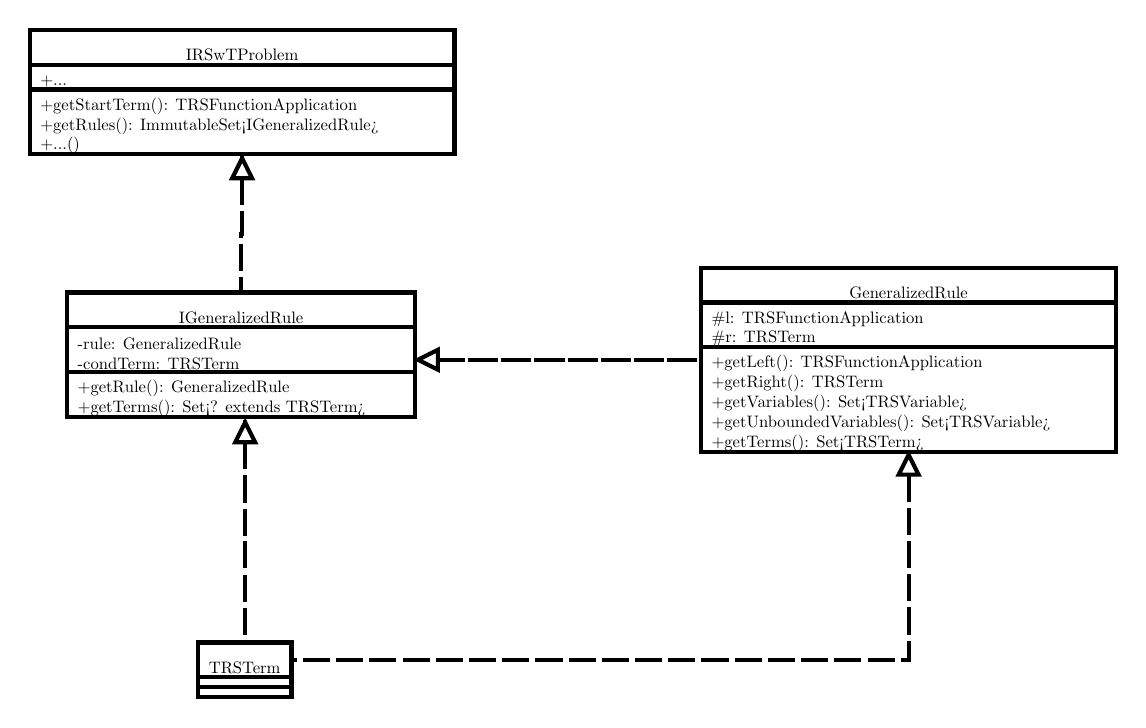
\begin{tikzpicture}[scale=0.6, every node/.style={scale=0.6}]
\pgftransformxscale{1.000000}
\pgftransformyscale{-1.000000}
\definecolor{dialinecolor}{rgb}{0.000000, 0.000000, 0.000000}
\pgfsetstrokecolor{dialinecolor}
\definecolor{dialinecolor}{rgb}{1.000000, 1.000000, 1.000000}
\pgfsetfillcolor{dialinecolor}
\pgfsetlinewidth{0.100000\du}
\pgfsetdash{}{0pt}
\definecolor{dialinecolor}{rgb}{1.000000, 1.000000, 1.000000}
\pgfsetfillcolor{dialinecolor}
\fill (9.250000\du,5.250000\du)--(9.250000\du,6.650000\du)--(26.305000\du,6.650000\du)--(26.305000\du,5.250000\du)--cycle;
\definecolor{dialinecolor}{rgb}{0.000000, 0.000000, 0.000000}
\pgfsetstrokecolor{dialinecolor}
\draw (9.250000\du,5.250000\du)--(9.250000\du,6.650000\du)--(26.305000\du,6.650000\du)--(26.305000\du,5.250000\du)--cycle;
% setfont left to latex
\definecolor{dialinecolor}{rgb}{0.000000, 0.000000, 0.000000}
\pgfsetstrokecolor{dialinecolor}
\node at (17.777500\du,6.250000\du){IRSwTProblem};
\definecolor{dialinecolor}{rgb}{1.000000, 1.000000, 1.000000}
\pgfsetfillcolor{dialinecolor}
\fill (9.250000\du,6.650000\du)--(9.250000\du,7.650000\du)--(26.305000\du,7.650000\du)--(26.305000\du,6.650000\du)--cycle;
\definecolor{dialinecolor}{rgb}{0.000000, 0.000000, 0.000000}
\pgfsetstrokecolor{dialinecolor}
\draw (9.250000\du,6.650000\du)--(9.250000\du,7.650000\du)--(26.305000\du,7.650000\du)--(26.305000\du,6.650000\du)--cycle;
% setfont left to latex
\definecolor{dialinecolor}{rgb}{0.000000, 0.000000, 0.000000}
\pgfsetstrokecolor{dialinecolor}
\node[anchor=west] at (9.400000\du,7.310000\du){+...};
\definecolor{dialinecolor}{rgb}{1.000000, 1.000000, 1.000000}
\pgfsetfillcolor{dialinecolor}
\fill (9.250000\du,7.650000\du)--(9.250000\du,10.250000\du)--(26.305000\du,10.250000\du)--(26.305000\du,7.650000\du)--cycle;
\definecolor{dialinecolor}{rgb}{0.000000, 0.000000, 0.000000}
\pgfsetstrokecolor{dialinecolor}
\draw (9.250000\du,7.650000\du)--(9.250000\du,10.250000\du)--(26.305000\du,10.250000\du)--(26.305000\du,7.650000\du)--cycle;
% setfont left to latex
\definecolor{dialinecolor}{rgb}{0.000000, 0.000000, 0.000000}
\pgfsetstrokecolor{dialinecolor}
\node[anchor=west] at (9.400000\du,8.310000\du){+getStartTerm(): TRSFunctionApplication};
% setfont left to latex
\definecolor{dialinecolor}{rgb}{0.000000, 0.000000, 0.000000}
\pgfsetstrokecolor{dialinecolor}
\node[anchor=west] at (9.400000\du,9.110000\du){+getRules(): ImmutableSet<IGeneralizedRule>};
% setfont left to latex
\definecolor{dialinecolor}{rgb}{0.000000, 0.000000, 0.000000}
\pgfsetstrokecolor{dialinecolor}
\node[anchor=west] at (9.400000\du,9.910000\du){+...()};
\pgfsetlinewidth{0.100000\du}
\pgfsetdash{}{0pt}
\definecolor{dialinecolor}{rgb}{1.000000, 1.000000, 1.000000}
\pgfsetfillcolor{dialinecolor}
\fill (10.750000\du,15.800000\du)--(10.750000\du,17.200000\du)--(24.725000\du,17.200000\du)--(24.725000\du,15.800000\du)--cycle;
\definecolor{dialinecolor}{rgb}{0.000000, 0.000000, 0.000000}
\pgfsetstrokecolor{dialinecolor}
\draw (10.750000\du,15.800000\du)--(10.750000\du,17.200000\du)--(24.725000\du,17.200000\du)--(24.725000\du,15.800000\du)--cycle;
% setfont left to latex
\definecolor{dialinecolor}{rgb}{0.000000, 0.000000, 0.000000}
\pgfsetstrokecolor{dialinecolor}
\node at (17.737500\du,16.800000\du){IGeneralizedRule};
\definecolor{dialinecolor}{rgb}{1.000000, 1.000000, 1.000000}
\pgfsetfillcolor{dialinecolor}
\fill (10.750000\du,17.200000\du)--(10.750000\du,19.000000\du)--(24.725000\du,19.000000\du)--(24.725000\du,17.200000\du)--cycle;
\definecolor{dialinecolor}{rgb}{0.000000, 0.000000, 0.000000}
\pgfsetstrokecolor{dialinecolor}
\draw (10.750000\du,17.200000\du)--(10.750000\du,19.000000\du)--(24.725000\du,19.000000\du)--(24.725000\du,17.200000\du)--cycle;
% setfont left to latex
\definecolor{dialinecolor}{rgb}{0.000000, 0.000000, 0.000000}
\pgfsetstrokecolor{dialinecolor}
\node[anchor=west] at (10.900000\du,17.860000\du){-rule: GeneralizedRule};
% setfont left to latex
\definecolor{dialinecolor}{rgb}{0.000000, 0.000000, 0.000000}
\pgfsetstrokecolor{dialinecolor}
\node[anchor=west] at (10.900000\du,18.660000\du){-condTerm: TRSTerm};
\definecolor{dialinecolor}{rgb}{1.000000, 1.000000, 1.000000}
\pgfsetfillcolor{dialinecolor}
\fill (10.750000\du,19.000000\du)--(10.750000\du,20.800000\du)--(24.725000\du,20.800000\du)--(24.725000\du,19.000000\du)--cycle;
\definecolor{dialinecolor}{rgb}{0.000000, 0.000000, 0.000000}
\pgfsetstrokecolor{dialinecolor}
\draw (10.750000\du,19.000000\du)--(10.750000\du,20.800000\du)--(24.725000\du,20.800000\du)--(24.725000\du,19.000000\du)--cycle;
% setfont left to latex
\definecolor{dialinecolor}{rgb}{0.000000, 0.000000, 0.000000}
\pgfsetstrokecolor{dialinecolor}
\node[anchor=west] at (10.900000\du,19.660000\du){+getRule(): GeneralizedRule};
% setfont left to latex
\definecolor{dialinecolor}{rgb}{0.000000, 0.000000, 0.000000}
\pgfsetstrokecolor{dialinecolor}
\node[anchor=west] at (10.900000\du,20.460000\du){+getTerms(): Set<? extends TRSTerm>};
\pgfsetlinewidth{0.100000\du}
\pgfsetdash{}{0pt}
\definecolor{dialinecolor}{rgb}{1.000000, 1.000000, 1.000000}
\pgfsetfillcolor{dialinecolor}
\fill (36.200000\du,14.800000\du)--(36.200000\du,16.200000\du)--(52.870000\du,16.200000\du)--(52.870000\du,14.800000\du)--cycle;
\definecolor{dialinecolor}{rgb}{0.000000, 0.000000, 0.000000}
\pgfsetstrokecolor{dialinecolor}
\draw (36.200000\du,14.800000\du)--(36.200000\du,16.200000\du)--(52.870000\du,16.200000\du)--(52.870000\du,14.800000\du)--cycle;
% setfont left to latex
\definecolor{dialinecolor}{rgb}{0.000000, 0.000000, 0.000000}
\pgfsetstrokecolor{dialinecolor}
\node at (44.535000\du,15.800000\du){GeneralizedRule};
\definecolor{dialinecolor}{rgb}{1.000000, 1.000000, 1.000000}
\pgfsetfillcolor{dialinecolor}
\fill (36.200000\du,16.200000\du)--(36.200000\du,18.000000\du)--(52.870000\du,18.000000\du)--(52.870000\du,16.200000\du)--cycle;
\definecolor{dialinecolor}{rgb}{0.000000, 0.000000, 0.000000}
\pgfsetstrokecolor{dialinecolor}
\draw (36.200000\du,16.200000\du)--(36.200000\du,18.000000\du)--(52.870000\du,18.000000\du)--(52.870000\du,16.200000\du)--cycle;
% setfont left to latex
\definecolor{dialinecolor}{rgb}{0.000000, 0.000000, 0.000000}
\pgfsetstrokecolor{dialinecolor}
\node[anchor=west] at (36.350000\du,16.860000\du){\#l: TRSFunctionApplication};
% setfont left to latex
\definecolor{dialinecolor}{rgb}{0.000000, 0.000000, 0.000000}
\pgfsetstrokecolor{dialinecolor}
\node[anchor=west] at (36.350000\du,17.660000\du){\#r: TRSTerm};
\definecolor{dialinecolor}{rgb}{1.000000, 1.000000, 1.000000}
\pgfsetfillcolor{dialinecolor}
\fill (36.200000\du,18.000000\du)--(36.200000\du,22.200000\du)--(52.870000\du,22.200000\du)--(52.870000\du,18.000000\du)--cycle;
\definecolor{dialinecolor}{rgb}{0.000000, 0.000000, 0.000000}
\pgfsetstrokecolor{dialinecolor}
\draw (36.200000\du,18.000000\du)--(36.200000\du,22.200000\du)--(52.870000\du,22.200000\du)--(52.870000\du,18.000000\du)--cycle;
% setfont left to latex
\definecolor{dialinecolor}{rgb}{0.000000, 0.000000, 0.000000}
\pgfsetstrokecolor{dialinecolor}
\node[anchor=west] at (36.350000\du,18.660000\du){+getLeft(): TRSFunctionApplication};
% setfont left to latex
\definecolor{dialinecolor}{rgb}{0.000000, 0.000000, 0.000000}
\pgfsetstrokecolor{dialinecolor}
\node[anchor=west] at (36.350000\du,19.460000\du){+getRight(): TRSTerm};
% setfont left to latex
\definecolor{dialinecolor}{rgb}{0.000000, 0.000000, 0.000000}
\pgfsetstrokecolor{dialinecolor}
\node[anchor=west] at (36.350000\du,20.260000\du){+getVariables(): Set<TRSVariable>};
% setfont left to latex
\definecolor{dialinecolor}{rgb}{0.000000, 0.000000, 0.000000}
\pgfsetstrokecolor{dialinecolor}
\node[anchor=west] at (36.350000\du,21.060000\du){+getUnboundedVariables(): Set<TRSVariable>};
% setfont left to latex
\definecolor{dialinecolor}{rgb}{0.000000, 0.000000, 0.000000}
\pgfsetstrokecolor{dialinecolor}
\node[anchor=west] at (36.350000\du,21.860000\du){+getTerms(): Set<TRSTerm>};
\pgfsetlinewidth{0.100000\du}
\pgfsetdash{{1.000000\du}{1.000000\du}}{0\du}
\pgfsetdash{{0.400000\du}{0.400000\du}}{0\du}
\pgfsetmiterjoin
\pgfsetbuttcap
{
\definecolor{dialinecolor}{rgb}{0.000000, 0.000000, 0.000000}
\pgfsetfillcolor{dialinecolor}
% was here!!!
\definecolor{dialinecolor}{rgb}{0.000000, 0.000000, 0.000000}
\pgfsetstrokecolor{dialinecolor}
\draw (24.725000\du,18.500000\du)--(25.575000\du,18.500000\du)--(36.150000\du,18.500000\du)--(36.200000\du,18.500000\du);
}
\definecolor{dialinecolor}{rgb}{0.000000, 0.000000, 0.000000}
\pgfsetstrokecolor{dialinecolor}
\draw (25.636803\du,18.500000\du)--(25.575000\du,18.500000\du)--(36.150000\du,18.500000\du)--(36.200000\du,18.500000\du);
\pgfsetmiterjoin
\definecolor{dialinecolor}{rgb}{1.000000, 1.000000, 1.000000}
\pgfsetfillcolor{dialinecolor}
\fill (25.636803\du,18.100000\du)--(24.836803\du,18.500000\du)--(25.636803\du,18.900000\du)--cycle;
\pgfsetlinewidth{0.100000\du}
\pgfsetdash{}{0pt}
\pgfsetmiterjoin
\definecolor{dialinecolor}{rgb}{0.000000, 0.000000, 0.000000}
\pgfsetstrokecolor{dialinecolor}
\draw (25.636803\du,18.100000\du)--(24.836803\du,18.500000\du)--(25.636803\du,18.900000\du)--cycle;
% setfont left to latex
\pgfsetlinewidth{0.100000\du}
\pgfsetdash{{0.400000\du}{0.400000\du}}{0\du}
\pgfsetdash{{0.400000\du}{0.400000\du}}{0\du}
\pgfsetmiterjoin
\pgfsetbuttcap
{
\definecolor{dialinecolor}{rgb}{0.000000, 0.000000, 0.000000}
\pgfsetfillcolor{dialinecolor}
% was here!!!
\definecolor{dialinecolor}{rgb}{0.000000, 0.000000, 0.000000}
\pgfsetstrokecolor{dialinecolor}
\draw (17.777500\du,10.300311\du)--(17.777500\du,13.450156\du)--(17.737500\du,13.450156\du)--(17.737500\du,15.800000\du);
}
\definecolor{dialinecolor}{rgb}{0.000000, 0.000000, 0.000000}
\pgfsetstrokecolor{dialinecolor}
\draw (17.777500\du,11.212115\du)--(17.777500\du,13.450156\du)--(17.737500\du,13.450156\du)--(17.737500\du,15.800000\du);
\pgfsetmiterjoin
\definecolor{dialinecolor}{rgb}{1.000000, 1.000000, 1.000000}
\pgfsetfillcolor{dialinecolor}
\fill (18.177500\du,11.212115\du)--(17.777500\du,10.412115\du)--(17.377500\du,11.212115\du)--cycle;
\pgfsetlinewidth{0.100000\du}
\pgfsetdash{}{0pt}
\pgfsetmiterjoin
\definecolor{dialinecolor}{rgb}{0.000000, 0.000000, 0.000000}
\pgfsetstrokecolor{dialinecolor}
\draw (18.177500\du,11.212115\du)--(17.777500\du,10.412115\du)--(17.377500\du,11.212115\du)--cycle;
% setfont left to latex
\pgfsetlinewidth{0.100000\du}
\pgfsetdash{}{0pt}
\definecolor{dialinecolor}{rgb}{1.000000, 1.000000, 1.000000}
\pgfsetfillcolor{dialinecolor}
\fill (16.000000\du,29.850000\du)--(16.000000\du,31.250000\du)--(19.757500\du,31.250000\du)--(19.757500\du,29.850000\du)--cycle;
\definecolor{dialinecolor}{rgb}{0.000000, 0.000000, 0.000000}
\pgfsetstrokecolor{dialinecolor}
\draw (16.000000\du,29.850000\du)--(16.000000\du,31.250000\du)--(19.757500\du,31.250000\du)--(19.757500\du,29.850000\du)--cycle;
% setfont left to latex
\definecolor{dialinecolor}{rgb}{0.000000, 0.000000, 0.000000}
\pgfsetstrokecolor{dialinecolor}
\node at (17.878750\du,30.850000\du){TRSTerm};
\definecolor{dialinecolor}{rgb}{1.000000, 1.000000, 1.000000}
\pgfsetfillcolor{dialinecolor}
\fill (16.000000\du,31.250000\du)--(16.000000\du,31.650000\du)--(19.757500\du,31.650000\du)--(19.757500\du,31.250000\du)--cycle;
\definecolor{dialinecolor}{rgb}{0.000000, 0.000000, 0.000000}
\pgfsetstrokecolor{dialinecolor}
\draw (16.000000\du,31.250000\du)--(16.000000\du,31.650000\du)--(19.757500\du,31.650000\du)--(19.757500\du,31.250000\du)--cycle;
\definecolor{dialinecolor}{rgb}{1.000000, 1.000000, 1.000000}
\pgfsetfillcolor{dialinecolor}
\fill (16.000000\du,31.650000\du)--(16.000000\du,32.050000\du)--(19.757500\du,32.050000\du)--(19.757500\du,31.650000\du)--cycle;
\definecolor{dialinecolor}{rgb}{0.000000, 0.000000, 0.000000}
\pgfsetstrokecolor{dialinecolor}
\draw (16.000000\du,31.650000\du)--(16.000000\du,32.050000\du)--(19.757500\du,32.050000\du)--(19.757500\du,31.650000\du)--cycle;
\pgfsetlinewidth{0.100000\du}
\pgfsetdash{{0.400000\du}{0.400000\du}}{0\du}
\pgfsetdash{{0.400000\du}{0.400000\du}}{0\du}
\pgfsetmiterjoin
\pgfsetbuttcap
{
\definecolor{dialinecolor}{rgb}{0.000000, 0.000000, 0.000000}
\pgfsetfillcolor{dialinecolor}
% was here!!!
\definecolor{dialinecolor}{rgb}{0.000000, 0.000000, 0.000000}
\pgfsetstrokecolor{dialinecolor}
\draw (17.900000\du,20.900000\du)--(17.900000\du,25.775000\du)--(17.878750\du,25.775000\du)--(17.878750\du,29.850000\du);
}
\definecolor{dialinecolor}{rgb}{0.000000, 0.000000, 0.000000}
\pgfsetstrokecolor{dialinecolor}
\draw (17.900000\du,21.811803\du)--(17.900000\du,25.775000\du)--(17.878750\du,25.775000\du)--(17.878750\du,29.850000\du);
\pgfsetmiterjoin
\definecolor{dialinecolor}{rgb}{1.000000, 1.000000, 1.000000}
\pgfsetfillcolor{dialinecolor}
\fill (18.300000\du,21.811803\du)--(17.900000\du,21.011803\du)--(17.500000\du,21.811803\du)--cycle;
\pgfsetlinewidth{0.100000\du}
\pgfsetdash{}{0pt}
\pgfsetmiterjoin
\definecolor{dialinecolor}{rgb}{0.000000, 0.000000, 0.000000}
\pgfsetstrokecolor{dialinecolor}
\draw (18.300000\du,21.811803\du)--(17.900000\du,21.011803\du)--(17.500000\du,21.811803\du)--cycle;
% setfont left to latex
\pgfsetlinewidth{0.100000\du}
\pgfsetdash{{0.400000\du}{0.400000\du}}{0\du}
\pgfsetdash{{0.400000\du}{0.400000\du}}{0\du}
\pgfsetmiterjoin
\pgfsetbuttcap
{
\definecolor{dialinecolor}{rgb}{0.000000, 0.000000, 0.000000}
\pgfsetfillcolor{dialinecolor}
% was here!!!
\definecolor{dialinecolor}{rgb}{0.000000, 0.000000, 0.000000}
\pgfsetstrokecolor{dialinecolor}
\draw (44.535000\du,22.200000\du)--(44.535000\du,30.550000\du)--(19.757500\du,30.550000\du);
}
\definecolor{dialinecolor}{rgb}{0.000000, 0.000000, 0.000000}
\pgfsetstrokecolor{dialinecolor}
\draw (44.535000\du,23.111803\du)--(44.535000\du,30.550000\du)--(19.757500\du,30.550000\du);
\pgfsetmiterjoin
\definecolor{dialinecolor}{rgb}{1.000000, 1.000000, 1.000000}
\pgfsetfillcolor{dialinecolor}
\fill (44.935000\du,23.111803\du)--(44.535000\du,22.311803\du)--(44.135000\du,23.111803\du)--cycle;
\pgfsetlinewidth{0.100000\du}
\pgfsetdash{}{0pt}
\pgfsetmiterjoin
\definecolor{dialinecolor}{rgb}{0.000000, 0.000000, 0.000000}
\pgfsetstrokecolor{dialinecolor}
\draw (44.935000\du,23.111803\du)--(44.535000\du,22.311803\du)--(44.135000\du,23.111803\du)--cycle;
% setfont left to latex
\end{tikzpicture}
